\documentclass[11pt]{article}
\usepackage[margin=1in]{geometry}
\usepackage[utf8]{inputenc}
\usepackage[T1]{fontenc}
\usepackage{lmodern}
\usepackage{amsmath,amssymb}
\usepackage{graphicx}
\usepackage{booktabs}
\usepackage{xcolor}
\usepackage[colorlinks=true,linkcolor=blue!60!black,citecolor=blue!60!black,urlcolor=blue!60!black]{hyperref}
\usepackage[numbers,sort&compress]{natbib}

\title{Small Quantum Classifiers Under Matched\\Classical and Hardware Tests:\\[0.3em]
\large Pre-Registered Benchmarks, Fourier Surrogates and IBM Heron Runs}
\author{Vivek Reddy\\\small Independent researcher\\\small \href{mailto:vvardhan00@gmail.com}{\texttt{vvardhan00@gmail.com}}}
\date{November 2026 \quad (workshop version of~\cite{reddy2026full})}

\begin{document}
\maketitle

\begin{abstract}
We test small quantum neural networks (QNNs) against classical models under matched conditions: classical baselines get the same inputs and are tuned by cross-validation, the final comparison is pre-registered on untouched data, and hardware runs are compared with noise-free simulation on identical inputs using exact shot-noise statistics.
On two text tasks, a 4-qubit QNN on sentence-encoder features is within about two points of tuned classical models and, over three seeds, has no higher point estimate than any of them (sentiment 0.766 vs.\ 0.769; CVE severity 0.708 vs.\ 0.720, a tie within a pre-set $\pm 3$-point margin; a ten-seed sensitivity analysis keeps the tie, with the QNN 0.9 points lower and the interval excluding zero); a 1.5-point gap seen during design did not replicate.
The circuit's output lies exactly in a 624-feature Fourier basis, and a classical model trained on that basis outperforms the QNN on CVE (0.727) and is inconclusive on sentiment (0.756).
On IBM's \texttt{ibm\_marrakesh}, no run's accuracy differs significantly from noise-free simulation, but the mean output shifts towards one class in every run; single executions on two further Heron devices show the same sign with larger shifts.
All code, results and job identifiers are archived.
\end{abstract}

\section{Introduction}
Claims of quantum advantage in machine learning are hard to evaluate without matched classical baselines~\cite{bowles2024better}. We ask a narrow question: for a small, trainable quantum classifier that runs on current hardware, does it differ from well-tuned classical models on the same inputs, and how much does real-device noise change its outputs?
Our contributions are:
(i) an evaluation protocol with matched inputs, tuned baselines and a pre-registered confirmatory test on untouched data (Section~\ref{sec:protocol});
(ii) evidence that the QNN is close to, but not better than, tuned classical models on two text tasks, together with an exact Fourier characterisation of what the circuit computes and a classical surrogate built on it (Section~\ref{sec:classical});
(iii) a repeated hardware study on fixed physical qubits with paired tests against noise-free simulation (Section~\ref{sec:hardware}).
A companion study of learning from quantum data (entanglement, phases and a two-copy purity test, including a 2-qubit hardware run) is in the full version~\cite{reddy2026full}.

\section{Evaluation protocol}\label{sec:protocol}
\begin{enumerate}
  \item \textbf{Same inputs.} Classical baselines (logistic regression and an RBF SVM; an MLP where noted) receive exactly the features encoded into the circuit.
  \item \textbf{Tuned baselines and a classical reference.} Same-feature baselines are tuned by 5-fold cross-validation on the training data only. We also report logistic regression on the full feature set and all training data.
  \item \textbf{Same inputs on hardware.} Device runs use a fixed random subset of the test set; they are compared only with the noise-free simulator on that subset.
  \item \textbf{Shot noise as the null hypothesis.} Prediction changes on hardware are compared with the exact distribution expected from finite sampling alone, and repeated in separate jobs.
  \item \textbf{Pre-registered confirmation.} Because the design was chosen with test-set feedback (below), the final text-task comparison is repeated once on untouched data, with the system, the analysis and the decision rules committed publicly before that data was downloaded.
\end{enumerate}
\paragraph{Disclosure.} The circuit design and feature-reduction method were chosen in exploratory runs that reported test-set accuracy; no separate validation set was held out for those choices. Test-set numbers obtained during design are therefore exploratory and are reported in the full version; the pre-registered evaluation in Table~\ref{tab:confirm} is the confirmatory result for the text tasks. Rule 3 was introduced after our first hardware chart placed 40-input device accuracy beside 200-input simulator accuracy, which made the device appear better than the simulator on one dataset.


\section{Quantum classifiers on classical data}\label{sec:classical}
\paragraph{Model.} Inputs are reduced to one feature per qubit and min--max scaled to $[0,\pi]$ using the training data. The circuit repeats, twice, an $R_Y(x_i)$ encoding layer followed by one trainable \texttt{RealAmplitudes} layer (data re-uploading~\cite{perezsalinas2020reuploading,schuld2021encoding}); the class is the measured value of qubit~0 (class~1 if $P(1) > 0.5$). Weights are initialised uniformly in $[-\pi,\pi]$ from the seed and trained with L-BFGS-B (at most 60 iterations, one start) on the cross-entropy of the exact simulated output probabilities, with one-hot labels. We used Qiskit~1.4~\cite{qiskit} and qiskit-machine-learning~0.8.

\paragraph{Text data and partitions.} Texts are embedded with all-MiniLM-L6-v2~\cite{reimers2019sbert} (384 dimensions) and reduced to four features with partial least squares (PLS), fitted on the full training split; the scalers are also fitted on training data only.
\emph{Sentiment}: Rotten Tomatoes sentence polarity~\cite{pang2005seeing}, the standard 8{,}530/1{,}066 train/test split, balanced; the 1{,}066-sentence validation split was never used until the confirmatory evaluation.
\emph{CVE severity}: 12{,}116 NVD descriptions with CVSS v3.1 scores, published 1~January--29~April 2024, labelled high/critical if the base score is at least 7.0, and split by publication date: training up to 9~April 2024 (9{,}692; 49.9\% high/critical), test after it (2{,}424; 42.2\%). The label shift explains the 0.578 majority-class baseline.
For each seed, the QNN and the same-feature baselines are trained on the same balanced random subset of 600 training texts; the full-embedding reference uses all training texts.

\paragraph{Confirmatory evaluation.} We then froze the system and scored it once on data no design decision had touched: the Rotten Tomatoes validation split, and all 13{,}432 CVEs with CVSS v3.1 scores published 1~May--28~August 2024 (47.9\% high/critical). The protocol, script and decision rules were committed before the data was downloaded (protocol: AGI \texttt{results/confirmatory/PROTOCOL.md}, commit \texttt{dda5f41}). The pre-registered primary contrast is the QNN minus CV-tuned logistic regression on the same features, averaged over seeds, with a 95\% interval from a crossed two-level percentile bootstrap: each replicate resamples the three seeds with replacement and, independently, the test items with replacement, applying the same item resample to every selected seed (10{,}000 replicates). The pre-registered rules were: on sentiment, the expected gap is confirmed if that interval lies entirely below zero; on CVE severity, a tie is confirmed if it lies entirely within $[-0.03, +0.03]$ (an equivalence margin in the spirit of two one-sided tests). Contrasts against the SVM and the full-embedding reference were declared secondary. Table~\ref{tab:confirm} gives the outcome. On sentiment the expected gap did not replicate: the QNN is within 0.3 points of tuned logistic regression, and the interval includes zero. On CVE severity the pre-registered tie is confirmed, but the QNN is now nominally below rather than ahead, and in a secondary contrast it is nominally 1.8 points below the tuned SVM (interval excludes zero; not adjusted for multiple comparisons). Taken together, on untouched data the QNN is within about two points of tuned classical models on the same four features and has no higher point estimate than any of them; its only interval excluding zero is the secondary, unadjusted contrast with the tuned SVM on CVE. In a sensitivity analysis specified before running but outside the protocol, ten training seeds instead of three give the same verdicts with narrower intervals: on sentiment the QNN and tuned logistic regression are level ($+0.001$, $[-0.011, +0.014]$); on CVE the tie within $\pm 3$ points holds, but the QNN is now below tuned logistic regression by an interval that excludes zero ($-0.009$, $[-0.016, -0.002]$). The per-seed results show that the order of the QNN and tuned logistic regression changes between seeds on both tasks. Unrounded differences are in the results files.

\begin{table}[h]
\centering
\small
\resizebox{\linewidth}{!}{%
\begin{tabular}{lcc}
\toprule
Confirmatory set (accuracy, mean $\pm$ std over 3 seeds) & Sentiment (1{,}066) & CVE severity (13{,}432) \\
\midrule
Majority class & 0.500 & 0.521 \\
QNN, 4 qubits & 0.766 $\pm$ 0.003 & 0.708 $\pm$ 0.009 \\
Logistic regression, same 4 features, CV-tuned & 0.769 $\pm$ 0.006 & 0.720 $\pm$ 0.004 \\
RBF SVM, same 4 features, CV-tuned & 0.767 $\pm$ 0.002 & 0.726 $\pm$ 0.005 \\
Logistic regression, full embedding, CV-tuned & 0.777 & 0.725 \\
\midrule
QNN $-$ tuned logistic regression [95\% CI] & $-0.003$ [$-0.017$, $+0.011$] & $-0.011$ [$-0.024$, $+0.003$] \\
QNN $-$ tuned SVM [95\% CI] & $-0.001$ [$-0.013$, $+0.012$] & $-0.018$ [$-0.031$, $-0.003$] \\
Pre-registered verdict & expected gap not confirmed & tie within $\pm 3$ points confirmed \\
\bottomrule
\end{tabular}}
\caption{Pre-registered confirmatory evaluation on untouched data (sample std over seeds; crossed two-level bootstrap intervals over seeds and items).}
\label{tab:confirm}
\end{table}

\paragraph{Dequantization check.} Because each input angle is encoded twice by $R_Y$, whose generator has eigenvalues $\pm\tfrac12$, every output of the circuit, for any weights, is a trigonometric polynomial $f(x) = \sum_{\omega} a_\omega \cos(\omega \cdot x) + b_\omega \sin(\omega \cdot x)$ with integer frequencies $\omega \in \{-2,\dots,2\}^4$~\cite{schuld2021encoding}: 312 frequency vectors up to sign, so 624 features plus a constant. We verified this numerically: a least-squares fit in this basis reproduces the trained seed-0 QNN on 2{,}000 random inputs to a maximum error of $3 \times 10^{-15}$, while a basis truncated to $\{-1,0,1\}^4$ misses by 0.3--0.4. We then trained purely classical surrogates on that basis~\cite{landman2022rff}, logistic regression with $C$ tuned by 5-fold cross-validation, on the same features and training texts as the QNN, under a protocol committed before running. On the untouched CVE set the surrogate scores $0.727$ against the QNN's $0.708$ (QNN minus surrogate $-0.018$, $[-0.030, -0.007]$), so the QNN is classically matched and in fact exceeded. On untouched sentiment it scores $0.756$ against $0.766$ ($+0.010$, $[-0.008, +0.029]$), which the pre-registered rule classes as inconclusive; plain logistic regression on the four features (0.769) is ahead of both there. Random subsets of 128 frequencies perform like the full basis. Cross-validation chose the smallest $C$ in the pre-set grid; a post-hoc rerun with a wider grid changes no result by more than 0.002. Two results should be kept apart. The representation result is exact: the circuit's output lies in this 624-feature Fourier span, so the circuit's output function is a linear combination of these classical features, whatever the trained weights. The predictive result is mixed: the trained surrogate outperforms the QNN on CVE and is inconclusive on sentiment. With 624 features and 600 training texts, cross-validation chose strong regularisation (5-fold CV accuracy at the chosen $C$: 0.72--0.77 per seed); the features are unscaled cosines and sines in $[-1, 1]$. A remaining sentiment edge over this particular surrogate would reflect how the two models are trained and regularised, not a quantum resource, since the function class is the same. Ten seeds give the same readings: the surrogate ahead on CVE, inconclusive on sentiment.

\paragraph{Design choices.} An ablation on breast cancer (three seeds, part of the exploratory benchmark, so descriptive) crosses encoding with re-uploading: replacing angle encoding with \texttt{ZZFeatureMap}~\cite{havlicek2019supervised} lowers accuracy by 24 points with re-uploading and 19 without, positive in all six seed-by-setting cells; other single changes, including 2 or 6 qubits instead of 4, move accuracy by at most 1.4 points. The encoding, not the qubit count, is what mattered here~\cite{perezsalinas2020reuploading,schuld2021encoding}.

\section{Real-hardware behaviour}\label{sec:hardware}
\paragraph{Setup.} We ran the trained sentiment and CVE models (seed 0) on IBM's 156-qubit Heron device \texttt{ibm\_marrakesh} through the free Open Plan, with \texttt{SamplerV2}, 1{,}024 shots and no error mitigation or dynamical decoupling. Each circuit was transpiled once with Qiskit's preset pass manager (optimisation level 1, \texttt{seed\_transpiler}=0), so every run used the same physical qubits (0--3); the compiled circuit has depth 37 with six CZ gates. At execution time the readout errors of these qubits were 0.006--0.024 and the CZ errors 0.0022--0.0027 (full snapshot and job identifiers in the archived results). For each task we drew a fixed, stratified random sample of 200 test inputs and ran it as separate jobs: three for CVE severity (two at 16:16 and 16:18~UTC, and one about three hours later at 19:22~UTC) and one for sentiment. The device's reported calibration of these qubits was the same for all three CVE runs, so the later run separates them in time but not across a recalibration.

\paragraph{Statistics.} For an input with noise-free probability $p$ and $N$ shots, the probability that sampling alone changes the prediction is the exact binomial tail
\begin{equation}
q(p) = \begin{cases} P(K \le N/2), & p > 1/2,\\ P(K > N/2), & p \le 1/2,\end{cases}\qquad K \sim \mathrm{Bin}(N, p).
\end{equation}
Under the null hypothesis that the device adds nothing beyond shot noise, every run draws fresh shots, so outcomes are independent across inputs and runs even though runs reuse the same inputs; the total number of changed predictions then follows a Poisson-binomial distribution, which we compute exactly by convolution. A fixed device bias alone would not make runs dependent; dependence across runs would require a shared run-level effect such as drift or environmental fluctuation, which the pooled test does not model, so we also give the test for each run alone. Accuracy on the device is compared with noise-free accuracy on the same inputs by an exact McNemar test per run. Bias is the mean signed difference between device and noise-free $P(\text{class }1)$, given per run with a 95\% bootstrap interval over inputs, and pooled with a two-level bootstrap that resamples runs and then inputs. The same threshold ($P > 0.5$) is used in simulation and on the device.

\begin{figure}[h]
\centering
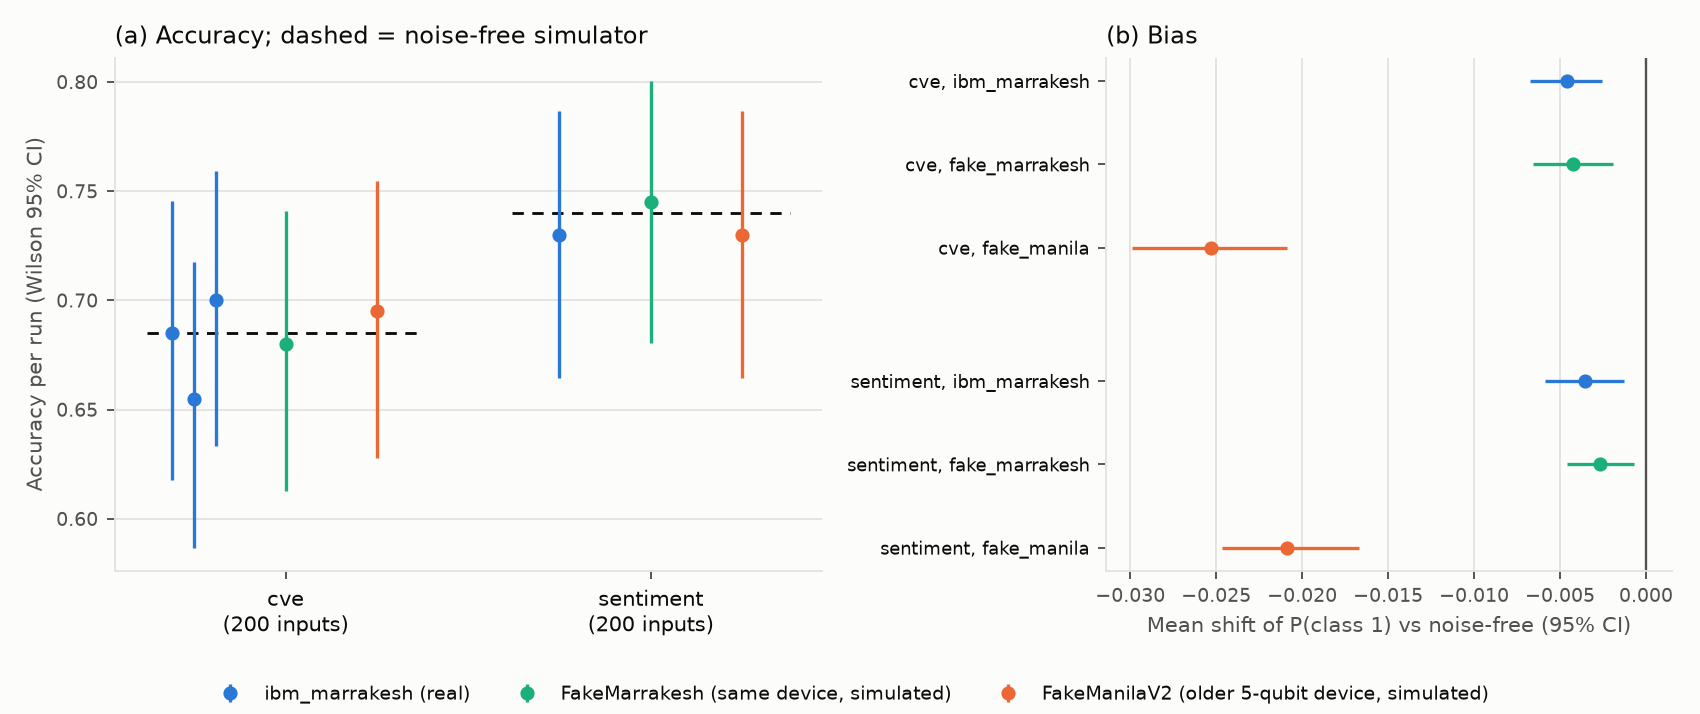
\includegraphics[width=\linewidth]{figures/agi_hardware_study.png}
\caption{Hardware study, 200 inputs per task. (a) Accuracy per run with Wilson 95\% intervals; dashed lines are noise-free accuracy on the same inputs. (b) Mean signed shift of $P(\text{class }1)$ relative to noise-free simulation, pooled over runs, with 95\% bootstrap intervals.}
\label{fig:hw}
\end{figure}

\paragraph{Results.} Figure~\ref{fig:hw} and Table~\ref{tab:hw} summarise the study. No run's accuracy differs significantly from noise-free accuracy on the same inputs: the three CVE runs score 0.685, 0.655 and 0.700 against a noise-free 0.685 (exact McNemar $p = 1$, $0.070$ and $0.45$; discordant pairs 2/2, 1/7 and 5/2), and sentiment scores 0.730 against 0.740 ($p = 0.63$). With 200 inputs this rules out only large accuracy changes. The numbers of changed predictions are at the edge of what shot noise explains: 19 against 13.3 expected over three CVE runs ($p = 0.055$; per run 4, 8 and 7 against 4.4, $p = 0.68$, $0.054$ and $0.13$), and 4 against 3.1 for sentiment ($p = 0.37$). We read this as compatible with shot noise, not as evidence of its absence. Repeated runs agree on 96\% of predictions. The mean output probability shifted towards class~0 in every run. For CVE the per-run shift was $-0.0063$ $[-0.0090, -0.0037]$ and $-0.0053$ $[-0.0081, -0.0025]$ in the first session and $-0.0022$ $[-0.0046, +0.0002]$ three hours later, whose interval includes zero; pooled over the three runs it is $-0.0046$, with a two-level interval of $[-0.0076, -0.0016]$. For sentiment (one run) it is $-0.0035$ $[-0.0061, -0.0010]$. The sign was the same in all four runs but the size varied between sessions, even under the same reported calibration, so we report a bias of these executions rather than a stable property of the device; the calibration snapshot records gate and readout error rates and coherence times, not drifts within a calibration cycle. Such a bias can change predictions for inputs near the decision boundary, so label agreement alone understates the effect of noise.

\begin{table}[h]
\centering
\small
\resizebox{\linewidth}{!}{%
\begin{tabular}{llcccc}
\toprule
Task & Backend & Accuracy per run & Changed / expected & $p$ & Bias [95\% CI] \\
\midrule
CVE (ideal 0.685) & \texttt{ibm\_marrakesh} & 0.685, 0.655, 0.700 & 19 / 13.3 & 0.055 & $-0.0046$ [$-0.0076$, $-0.0016$] \\
 & FakeMarrakesh & 0.680 & 3 / 4.4 & 0.86 & $-0.0043$ [$-0.0066$, $-0.0019$] \\
 & FakeManilaV2 & 0.695 & 12 / 4.4 & $<0.001$ & $-0.0253$ [$-0.0299$, $-0.0209$] \\
Sentiment (ideal 0.740) & \texttt{ibm\_marrakesh} & 0.730 & 4 / 3.1 & 0.37 & $-0.0035$ [$-0.0059$, $-0.0013$] \\
 & FakeMarrakesh & 0.745 & 3 / 3.1 & 0.63 & $-0.0027$ [$-0.0046$, $-0.0007$] \\
 & FakeManilaV2 & 0.730 & 8 / 3.1 & 0.003 & $-0.0209$ [$-0.0246$, $-0.0167$] \\
\bottomrule
\end{tabular}}
\caption{Hardware study, 200 inputs per task, 1{,}024 shots. ``Changed / expected'' counts predictions that differ from the noise-free prediction, against the exact shot-noise expectation; $p = P(\text{total} \ge \text{observed})$ under shot noise alone. Bias intervals are 95\% bootstraps over inputs (over runs and inputs for the three CVE runs); per-run values are in the text.}
\label{tab:hw}
\end{table}

\paragraph{Noise models.} \texttt{FakeMarrakesh}, Qiskit's noise model built from a calibration snapshot of the same device, agrees with the real device in accuracy behaviour and in the size of its bias: their difference lies within the intervals, while the bias itself is non-zero. \texttt{FakeManilaV2}, a model of an older 5-qubit device, overstates the bias about fivefold and changes significantly more predictions than shot noise allows. This compares two specific noise models on one circuit; it suggests matching the noise model to the device, rather than a general statement about noise models, and the next paragraph shows that even a same-device model can miss.

{\sloppy\paragraph{Other devices.} The Open Plan gives access to two further 156-qubit Heron r2 devices, \texttt{ibm\_kingston} and \texttt{ibm\_fez}. With the remaining quantum time we ran the CVE model once on each, on a 100-input stratified sample that is a subset of the 200 inputs above, compiled in the same way (both used physical qubits 0--3 with the same depth-37, six-CZ circuit). Table~\ref{tab:xdev} compares all three devices on these 100 inputs. No device's accuracy differs significantly from noise-free (exact McNemar $p \ge 0.13$ for every run), and the changed predictions on the two new devices are within shot noise. Every execution shifts the output towards class~0, but by different amounts: on the same inputs the \texttt{ibm\_fez} execution shifts it by $0.010$ more than \texttt{ibm\_marrakesh} (paired 95\% CI $[0.006, 0.015]$) and by $0.007$ more than \texttt{ibm\_kingston} ($[0.002, 0.011]$). \texttt{FakeFez} understates the shift on \texttt{ibm\_fez} by $0.006$ ($[0.002, 0.010]$), while \texttt{FakeMarrakesh} matches \texttt{ibm\_marrakesh} (difference $+0.0005$, $[-0.003, +0.004]$); no noise model of \texttt{ibm\_kingston} is distributed with Qiskit. These intervals are over inputs, conditional on the particular executions; with one run on each new device they describe these executions, not persistent device properties. The sign of the shift was the same in every execution, its size differed between them, and a same-device noise model matched \texttt{ibm\_marrakesh} but understated the \texttt{ibm\_fez} execution. One run per new device cannot separate device from session effects.\par}

\begin{table}[h]
\centering
\small
\resizebox{\linewidth}{!}{%
\begin{tabular}{lcccc}
\toprule
Backend (100 inputs; noise-free 0.650) & Accuracy & Changed / expected & $p$ & Mean shift [95\% CI] \\
\midrule
\texttt{ibm\_marrakesh}, 3 runs & 0.650, 0.600, 0.660 & 4, 7, 5 / 3.1 & -- & $-0.0050$ (per run $-0.007$, $-0.007$, $-0.002$) \\
\texttt{ibm\_kingston}, 1 run & 0.630 & 2 / 3.1 & 0.85 & $-0.0087$ [$-0.0121$, $-0.0055$] \\
\texttt{ibm\_fez}, 1 run & 0.640 & 5 / 3.1 & 0.17 & $-0.0152$ [$-0.0208$, $-0.0095$] \\
\texttt{FakeMarrakesh} & 0.660 & 1 / 3.1 & 0.97 & $-0.0045$ [$-0.0078$, $-0.0012$] \\
\texttt{FakeFez} & 0.640 & 3 / 3.1 & 0.63 & $-0.0092$ [$-0.0135$, $-0.0049$] \\
\bottomrule
\end{tabular}}
\caption{Cross-device replication of the CVE classifier on 100 identical inputs (a subset of Table~\ref{tab:hw}'s inputs); \texttt{ibm\_marrakesh} rows are its three runs restricted to these inputs. $p = P(\text{changed} \ge \text{observed})$ under shot noise alone.}
\label{tab:xdev}
\end{table}


\section{Quantum data (summary)}\label{sec:quantum}
The full version~\cite{reddy2026full} reports a second project in which models access quantum states directly. In exact simulation a trained two-copy QNN separates pure from mixed states with 16--32 copies per state from 2 to 6 qubits, against 128--4{,}096 for a classical-shadow baseline~\cite{huang2020shadows}, a small-scale illustration of known multi-copy separations~\cite{huang2022experiments,chen2021memory}. In a preliminary 2-qubit hardware run on one shared 60-state set, the QNN's estimated copy ratio is above 1 in both jobs, with intervals too broad to establish whether noise reduces the advantage. Entanglement and phase tasks did not separate quantum from classical models.

\section{Related work}
\textbf{Benchmarking.} Bowles et al.~\cite{bowles2024better} benchmark QML models at scale and find that classical baselines often match or beat them; our protocol follows the same spirit at small scale, adding hardware. \textbf{Encoding and expressivity.} Data re-uploading~\cite{perezsalinas2020reuploading} and the Fourier view of encoding~\cite{schuld2021encoding} explain why the encoding dominated our ablation. \textbf{Dequantization.} Quantum-inspired classical algorithms~\cite{tang2019dequantized} and random-Fourier-feature approximations of variational QML models~\cite{landman2022rff} suggest that circuits like ours may be classically approximable; our dequantization check (Section~\ref{sec:classical}) shows that our classifier's function class is exactly such a Fourier model; a classical surrogate on it outperforms the QNN on one task and is inconclusive on the other. \textbf{Hardware characterisation.} Capability benchmarks~\cite{proctor2022capabilities} and error mitigation~\cite{temme2017mitigation} address device noise systematically; we used no error mitigation and characterise only the output bias and accuracy of one shallow circuit.


\section{Discussion and limitations}
On classical data the circuit classifies features chosen by a classical encoder, tuned classical models on the same features do as well or slightly better, and the circuit's output lies in a Fourier basis that a classical learner can use directly, where it does at least as well on CVE.

Limitations: (i) the circuits use 4 qubits and are simulated exactly, so nothing here is classically hard; (ii) design choices were explored with test-set feedback (Section~\ref{sec:protocol}), which the confirmatory evaluation addresses only for the two text tasks; (iii) the ablation uses one dataset, itself part of the exploratory benchmark; (iv) the hardware study uses one circuit family on three devices of one processor family, with 200 inputs and few runs on one device and a single 100-input CVE run on each of the others, and the bias may drift with calibration; (v) prediction changes are tested under an independence assumption across inputs and runs; (vi) CVE severity from descriptions alone approximates CVSS scoring; (vii) the pre-registered text-task verdicts rest on three training seeds (a ten-seed sensitivity analysis gives the same verdicts). Limitations of the quantum-data study are discussed in the full version~\cite{reddy2026full}.

\paragraph{Reproducibility.} Code, configurations, result files and job identifiers are archived on Zenodo as AGI v1.0.5~\cite{reddy2026agi} (git commit \texttt{d48ebde}) and Entangle v1.0.1~\cite{reddy2026entangle} (git commit \texttt{21ab264}), with the DOIs given in the references; every number in this paper comes from these versions. The full version lists software versions, commands and job identifiers. During this work we found that \texttt{qiskit-ibm-runtime}~0.44.1 declares Qiskit~1.x support but fails to transpile for real devices on it; we reported it upstream (Qiskit/qiskit-ibm-runtime\#3563).

\paragraph{Acknowledgements.} Code, experiments and drafting were carried out with assistance from an AI coding assistant (Claude, Anthropic); an independent critical review was obtained from another AI model (ChatGPT, OpenAI). The author reviewed all results and takes responsibility for the content. We thank IBM Quantum for Open Plan access.

\bibliographystyle{unsrtnat}
\bibliography{refs}
\end{document}
